\tikzstyle{end} = [circle, minimum size = 0.1cm, draw, inner sep = 0.1pt]
\tikzstyle{leaf} = [circle, minimum size = 0.6cm, draw, inner sep = 0.1pt, blue]


\onslide<1->{
	\tikzstyle{level 1}=[level distance = 1.5cm, sibling distance = 6cm, opacity = 0]
	\tikzstyle{level 2}=[sibling distance = 3cm, opacity = 0]
}
\only<3->{
	\tikzstyle{level 1}=[level distance = 1.5cm, sibling distance = 6cm, opacity = 1]
	\tikzstyle{level 2}=[sibling distance = 3cm, opacity = 1]
}






    
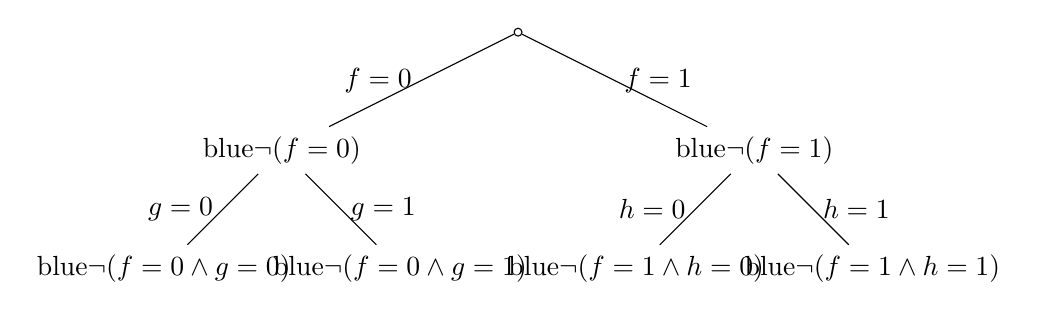
\begin{tikzpicture}[label distance = 8mm, all/.style = {opacity = 0}]
	\node [end] {}
        child {
            node {\mycolor{blue}{$\neg (f = 0)$}}
           	child {
                node {\mycolor{blue}{$\neg (f = 0 \land g = 0)$}}
                edge from parent
	            node[left] {$g = 0$}
            }
            child {
               	node {\mycolor{blue}{$\neg (f = 0 \land g = 1)$}}
                edge from parent
	            node[right] {$g = 1$}
            }
           	edge from parent
            node[left] {$f = 0$}
        }
        child {
            node {\mycolor{blue}{$\neg (f = 1)$}}
           	child {
                node {\mycolor{blue}{$\neg (f = 1 \land h = 0)$}}
                edge from parent
	            node[left] {$h = 0$}
            }
            child {
               	node {\mycolor{blue}{$\neg (f = 1 \land h = 1)$}}
                edge from parent
	            node[right] {$h = 1$}
            }
           	edge from parent
            node[right] {$f = 1$}
        };
\end{tikzpicture}

%%% Local Variables: 
%%% mode: latex
%%% TeX-master: t
%%% End: 
